\documentclass{article}
\usepackage[final,nonatbib]{project}
% This MiKTeX release clashes on the two theorem environments that share the
% theorem counter; defining the names first makes watml.sty skip them, so the
% course style file itself stays unmodified.
\providecommand{\axiom}{}\providecommand{\claim}{}
\usepackage{watml}
\usepackage[normalem]{ulem}
\usepackage{setspace}
\usepackage{times}
\usepackage{graphicx}
\usepackage{array}
\graphicspath{{results/report/}{results/final/}}
\addbibresource{references.bib}
\ExecuteBibliographyOptions{dashed=false}
\DeclareFieldFormat[article]{eid}{Article~#1}
% Every result quoted in the text is a macro written by a script from the
% saved measurements: the course study (results/final), the extended study
% (results/paper/final) and the report's own figures and tables
% (results/report), all evaluated on the same Linux server, and every count of
% the data by the script that collected it.
\newcommand{\inputif}[1]{\IfFileExists{#1}{\input{#1}}{}}
\inputif{results/final/numbers.tex}
\inputif{results/runs/compare_M1_M3.tex}
\inputif{queries/tpcds_sf1/query_numbers.tex}
\inputif{results/tpcds_sf1/screen_numbers.tex}
\inputif{results/paper/final/numbers.tex}
\inputif{results/paper/final/operators.tex}
\inputif{results/paper/final/sources.tex}
\inputif{results/paper/final/streams.tex}
\inputif{results/paper/final/single_run.tex}
\inputif{results/report/numbers.tex}
% Let a page take two floats on top before the text, as long as some text stays.
\renewcommand{\topfraction}{0.8}
\renewcommand{\textfraction}{0.15}
\setcounter{topnumber}{3}
% The public repository with the code and data, without https://; the abstract prints the link once it is set.
\newcommand{\codeurl}{github.com/KrishPatel13/query-runtime-transfer}

\makeatletter
\renewcommand{\@noticestring}{CS680 (Fall 2026). Project Report. Krish Patel}
\makeatother

\title{Adapting Small Query Runtime Models\\to New Machines and Unseen Query Templates}
\author{Krish Patel\\
Email: \texttt{kmp.patel@uwaterloo.ca}\\
CS 680: Introduction to Machine Learning, University of Waterloo}
\date{}

\begin{document}
\maketitle

\begin{abstract}
Query runtime models are trained on one machine and drift when the hardware changes. For small models that predict PostgreSQL runtime from 19 plan features, I ask how many queries measured on a new machine suffice to adapt them (Q1), and whether a model anchored to the optimizer's cost predicts runtime for templates it never saw (Q2). I timed 1,162 TPC-H and TPC-DS queries in six environments with identical plans. The slowdown varies mostly between templates, so a speed factor from five measured queries removes much of the error and then stops improving. A ridge regression of the old model's errors keeps improving on TPC-H: in Q1's primary test its error at 25 queries is \PrimaryGeo{} times the speed factor's (95\% interval \PrimaryGeoLo{} to \PrimaryGeoHi). A per-template correction from one measured query per template does better on both benchmarks (error \PLadTpchLowdimTemplateRoundRobin{} on TPC-H, \PLadTpcdsLowdimTemplateRoundRobin{} on TPC-DS), close to the same correction on a model trained on the new machine. On unseen templates nothing reliably beats the speed factor, and Q2's primary test fails (ratio to the cost line \CFourGeo, interval \CFourGeoLo{} to \CFourGeoHi).\ifx\codeurl\empty\else{} Code and data: \href{https://\codeurl}{\nolinkurl{\codeurl}}.\fi
\end{abstract}

\section{Introduction}
A database system that knows how long a query will take can route short queries past long ones, hold back a query that would take hours, and size a cluster for a workload. PostgreSQL's optimizer estimates a cost for every plan, but in units whose relation to time depends on the machine and the plan \parencite{wu2013}. Learned models close this gap by mapping plan features to measured runtime \parencite{ganapathi2009,akdere2012,marcus2019}, and production systems use such predictions for scheduling \parencite{wu2024stage}.

A learned runtime model is trained on one machine. Move the database to other hardware, or give it fewer processors, and the same plans change speed by different factors (Figure~\ref{fig:overview}a). In machine-learning terms the inputs do not change: the same queries get the same plans and features everywhere, so the input distribution is fixed and only the distribution of runtime given the features shifts. Reweighting unlabeled inputs, the usual answer to covariate shift \parencite{shimodaira2000}, has nothing to correct; the model needs runtimes measured on the new machine, and each costs time there. The first question (Q1) is one of few-shot adaptation: how few queries measured on a target machine are enough to adapt a model trained on a source machine, which queries should they be, and does it keep improving as more arrive? The second (Q2) asks whether a model anchored to the optimizer's cost predicts runtime for templates never seen in training, which earlier work found hard for plan-level models \parencite{akdere2012}; each template acts as a domain. The contributions are:
\begin{itemize}[leftmargin=*,itemsep=0pt,topsep=2pt]
\item a dataset of 1,162 TPC-H and TPC-DS queries timed in three passes in six environments with identical plans (I found no public dataset that times the same plans on several machines), and an analysis of how their runtimes shift;
\item for Q1, the primary test, in which a ridge correction of the source model's errors beats one speed factor, and an extension in which per-template offsets from one query per template come close to a model trained on the target, confirmed on \PHPairs{} pairs measured after five hypotheses were fixed;
\item for Q2, a negative result: on templates without measured queries no correction reliably beats the speed factor, and the cost-anchored model is no better than a line on the optimizer's cost.
\end{itemize}

\begin{figure}[t]
\centering
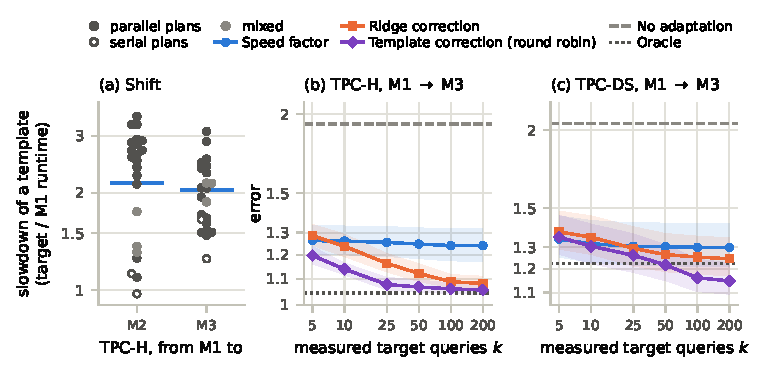
\includegraphics[width=\textwidth]{fig_overview.pdf}
\caption{(a) Slowdown of each TPC-H template from M1 to M2 (one processor) and to M3 (the server): filled if all its plans have parallel workers, hollow if none, gray if mixed; the blue line is the geometric mean, the factor a speed factor estimates. (b, c) Error (Section~\ref{sec:setup}) against the number $k$ of measured target queries from M1 to M3, with 95\% intervals over templates.}
\label{fig:overview}
\end{figure}

\section{Related Work}
\textbf{Runtime models and new hardware.} Plan-level models predict runtime from plan features \parencite{ganapathi2009} but transfer poorly to a held-out template \parencite{akdere2012}; plan-structured networks \parencite{marcus2019}, tree models \parencite{sun2020} and tree transformers \parencite{zhao2022} train on thousands of queries, explicit features on far fewer \parencite{yu2023}, and all inherit wrong row estimates \parencite{leis2015}. For a new machine, \textcite{wu2013} calibrate PostgreSQL's cost units with designed queries, \textcite{zhu1994} fit a cost formula per query class from sampled queries, and ParamTree predicts cost constants from hardware and settings \parencite{yang2023}; zero-shot models transfer across databases on one machine \parencite{hilprecht2022}. QCFE retrains on 200 rerun queries \parencite{yan2024qcfe}, DACE fine-tunes on a whole rerun workload \parencite{liang2024dace}, T3 reruns its benchmark \parencite{rieger2025t3}, and Redshift feeds the instance type to a global model \parencite{wu2024stage}. These need many target queries or a description of the hardware; I ask how few measured queries suffice, and which.

\textbf{Transferring and updating models.} For configurable software, a line from source to target performance (model shift) moves a model across hardware with 5 to 15 runs \parencite{valov2017,jamshidi2017} and fails for severe changes \parencite{valov2020,jamshidi2018}; OneProxy adapts a latency predictor with one global factor plus sparse per-operator deviations \parencite{lu2021oneproxy}. Clinical prediction calls the speed factor \emph{recalibration in the large} and finds it hard to beat unless the new sample is large \parencite{steyerberg2004,vergouwe2017}. \textcite{kuzborskij2013} analyze least squares regularized toward a source hypothesis, which my ridge correction is; learning the residuals of an analytical model follows \textcite{didona2015}; and learned database models have been updated for shifts in data and workload \parencite{kurmanji2023,wui2024}.

\textbf{Choosing what to measure.} Farthest-first selection covers a feature space \parencite{gonzalez1985,sener2018}, D-optimal design pins down a linear model \parencite{wynn1970,mitchell1974}, and Ernest picks training runs by optimal design under a cost budget \parencite{venkataraman2016ernest}. Streams are scored test-then-train \parencite{gama2013}. I claim only prediction accuracy, since better predictions need not give better plans \parencite{heinrich2025}.

\section{Problem Setup}
\label{sec:setup}
For a query $q$ from template $\tau(q)$ (one SQL text whose queries differ only in parameters), let $x(q)\in\mathbb{R}^{19}$ be the features of plain \texttt{EXPLAIN} \parencite{postgresExplain}: estimated startup and total cost, rows and width; node count and depth; the largest and summed log row estimates over nodes; counts of scans, joins, sorts, aggregates, materializations and subplans by type; and planned parallel workers. Let $y_m(q)$ be its runtime in environment $m$. The plan, and so $x(q)$, is the same in every environment (Section~\ref{sec:experiments}). Models predict $\log y$; accuracy is the Q-error $Q(y,\hat y)=\max(y/\hat y,\hat y/y)$ \parencite{moerkotte2009}.

\textbf{The shift.} On a target $t$, a source model $f_s$ trained on environment $s$ has log error $e(q)=\log y_t(q)-f_s(x(q))=\delta(q)+u_s(q)$: the log slowdown $\delta(q)=\log(y_t(q)/y_s(q))$ plus the model's residual $u_s(q)$ on the source. The corrections below assume $\delta$ is a constant (speed factor), a function of $x$ (ridge correction) or a value per template (template offsets). The template share
\begin{equation}
\eta^2=\textstyle\sum_{\tau} n_\tau(\bar\delta_\tau-\bar\delta)^2\big/\sum_q(\delta(q)-\bar\delta)^2,
\label{eq:share}
\end{equation}
with $n_\tau$ queries of mean slowdown $\bar\delta_\tau$ in template $\tau$, is the part of the variance of $\delta$ between templates; computed between two passes on one machine, it measures noise.

\textbf{Q1 and Q2.} Queries are split once, inside every template, into a pool $P$ and a test set $T$ with templates $\mathcal T$, the same in every environment. A selection rule picks $k$ pool queries without running them on the target; their target runtimes and $f_s$ give the adapted model $f_t$, scored on $T$. Random selection follows one of $R=\EvalOrders$ arrival orders shared by all methods. For Q2, models are trained without a template $g$ (TPC-DS: its family of near copies) and scored on $g$.

\textbf{Metrics.} For a method, a $k$ and an order $r$, each test template gets the median Q-error $\tilde Q_{\tau r}$ of its test queries; the error
\begin{equation}
E(k)=\exp\Bigl(\tfrac{1}{|\mathcal T|}\textstyle\sum_{\tau\in\mathcal T}\tfrac1R\sum_{r=1}^R\log\tilde Q_{\tau r}\Bigr)
\end{equation}
is a geometric mean in which every test template counts once. Two methods are compared by the geometric mean over templates of the ratio of their errors, with a 95\% interval from \EvalBootstrap{} resamples of whole templates (TPC-DS: families) \parencite{efron1993}, paired across methods. With $E_{\mathrm{none}}$ for the unadapted model and $E_{\mathrm{oracle}}$ for the source pipeline retrained on the whole target pool, $G(k)=\log(E_{\mathrm{none}}/E(k))/\log(E_{\mathrm{none}}/E_{\mathrm{oracle}})$ is the share of the gap closed. The oracle knows nothing of templates, so it is a reference, not a bound ($G>1$ is possible).

\section{Methods}
\label{sec:methods}
\textbf{Source models.} The \emph{cost line} regresses log runtime on $\log(1+\kappa(x))$, with $\kappa(x)$ PostgreSQL's total cost; \emph{ridge regression} \parencite{hoerl1970} uses the standardized features; the \emph{random forest} \parencite{breiman2001} has 300 trees, two samples per leaf and $\sqrt{19}$ features per split; and the \emph{correction model}, fixed before the study as $f_s$, adds a random forest on the cost line's residuals, so that it falls back to the cost line where the forest learned little. The template and global means ignore the plan. All use scikit-learn \parencite{pedregosa2011}.

\textbf{Corrections.} With $e_i$ the source model's log error on the $k$ measured queries and $\bar e$ their mean, each correction predicts $\log\hat y=f_s(x)+c(x)$:
\begin{itemize}[leftmargin=*,itemsep=0pt,topsep=2pt]
\item \emph{Speed factor}: $c=\bar e$, one factor on runtime.
\item \emph{Ridge correction}: $c(x)=\hat\beta_0+\hat\beta^\top\tilde x$, with $\tilde x$ the features standardized over the $k$ queries and
\begin{equation}
(\hat\beta_0,\hat\beta)=\arg\min_{\beta_0,\beta}\ \textstyle\sum_{i=1}^k\bigl(e_i-\beta_0-\beta^\top\tilde x_i\bigr)^2+\lambda\|\beta\|^2,
\label{eq:ridgecorr}
\end{equation}
the intercept unpenalized and $\lambda$ chosen by leave-one-out \parencite{golub1979} among 45 values from $10^{-6}$ to $10^{5}$.
\item \emph{Affine+parallel}: $c(x)=a+b\,f_s(x)+\pi(x)(a'+b'f_s(x))$, with $\pi(x)=1$ for plans with parallel workers, fitted like \eqref{eq:ridgecorr} with 2 to 4 parameters.
\item \emph{Template offsets} and the \emph{template correction}: the speed factor, or affine+parallel, plus for each measured template the mean residual of its queries; other templates get the factor or line alone.
\item \emph{1-NN}: the error of the nearest measured query in the standardized feature space, without template labels.
\end{itemize}
As baselines, \emph{target only} trains the source pipeline on the $k$ queries, the \emph{pooled refit} on the source pool plus the $k$ queries with the environment as a feature, the \emph{forest on the errors} fits a forest to the $e_i$, the \emph{template lookup} predicts a template's mean measured log runtime, and the \emph{oracle} trains on the whole target pool. The \emph{no-move control} applies a correction to a model trained on the target pool itself, so the gap to it is the cost of the move.

\begin{proposition}\label{prop:limit}
For every $\lambda>0$, the solution of \eqref{eq:ridgecorr} has $\hat\beta_0=\bar e$ and $\hat\beta=(\tilde X^\top\tilde X+\lambda I)^{-1}\tilde X^\top(e-\bar e\mathbf 1)$, where $\tilde X$ stacks the $\tilde x_i$, and $\|\hat\beta\|\le\|\tilde X^\top(e-\bar e\mathbf 1)\|/\lambda$. Hence as $\lambda\to\infty$ the ridge correction becomes the speed factor.
\end{proposition}
\begin{proof}
The standardized features sum to zero over the $k$ queries, so the derivative in $\beta_0$ gives $k\beta_0=\sum_i e_i-\beta^\top\sum_i\tilde x_i=k\bar e$. Then $\beta$ minimizes $\|(e-\bar e\mathbf 1)-\tilde X\beta\|^2+\lambda\|\beta\|^2$, with the stated unique minimizer, and the eigenvalues of $(\tilde X^\top\tilde X+\lambda I)^{-1}$ are at most $1/\lambda$ since $\tilde X^\top\tilde X$ is positive semidefinite.
\end{proof}
The speed factor is one end of the ridge correction's family, and leave-one-out picks the point the $k$ queries support, noisily when $k$ is as small as 5. Template offsets put all their freedom in the templates instead.

\textbf{Choosing the $k$ queries.} \emph{Random} follows the arrival order. \emph{Round robin} takes one query of each template in turn, in random order; \emph{cheapest per template} is round robin from each template's fastest source query. \emph{k-center} adds the query farthest from those chosen in the standardized feature space \parencite{gonzalez1985,sener2018}, \emph{D-optimal} the one that most increases $\det(I+X^\top X)$ \parencite{wynn1970,mitchell1974}, and \emph{plan class} alternates parallel and serial plans. Each rule derives its $r$-th sequence from the $r$-th order, so comparisons are paired. Algorithm~\ref{alg:adapt} combines the pieces.

\begin{algorithm}[t]
\small
\DontPrintSemicolon
\KwIn{source model $f_s$; target pool $P$; selection rule; correction $c$; budget $k$; window $W$ (all, or 50)}
$S\gets$ the first $k$ queries chosen from $P$ \tcp*{before any target run}
run each $q\in S$ on the target; $e_q\gets\log y_t(q)-f_s(x(q))$\;
fit $c$ to $\{(x(q),\tau(q),e_q):q\in S\}$; $f_t\gets f_s+c$ \tcp*{C2 ends here}
\For{each later batch $B$ of queries}{
  predict $f_t$ on $B$, run $B$, add it to $S$ \tcp*{test-then-train}
  refit $c$ on the last $W$ queries of $S$ \tcp*{C3}
}
\caption{Adapting a source model with measured target queries and continuing to learn}
\label{alg:adapt}
\end{algorithm}

\section{Experimental Setup}
\label{sec:experiments}
\textbf{Environments} (Table~\ref{tab:envs}). M2, M4 and M6 pin every PostgreSQL process to one or two virtual processors, which a plan's leader and parallel workers (at most two per Gather node) then share; the proposal limited all of WSL instead, but pinning changes only the database's processors. All run PostgreSQL 18.6 from one build, without JIT, with one set of settings apart from M5's buffer pool, on copies of M1's database files, so every saved plan, with its estimates, is identical in all six. The data fit in memory everywhere. The proposal planned M1 to M3 and TPC-DS on M1 (the course study); the extended study added the rest.

\begin{table}[t]
\caption{The six environments. Pass: minutes for one pass over a workload (median of three). Noise: Q-error between two passes over the same query, median / 90th percentile.}
\label{tab:envs}
\centering\small
\inputif{results/report/table_envs.tex}
\end{table}

\textbf{Workloads.} TPC-H at scale factor 1 \parencite{tpch}: 680 queries from 22 templates, the 420 of an earlier pilot plus 20 with widened ranges for each of the 13 templates with range parameters, so that runtime varies inside a template. TPC-DS at scale factor 1 \parencite{tpcds}: up to 5 parameter draws per template, with templates over 30\,s in a screening run on M1 dropped before any label existed, which leaves \DSScreenCollectFiles{} queries from \DSScreenKeptGroups{} templates. Templates whose first queries share at least 85\% of their tokens are near copies (37 and 82 differ only in the sales channel) and form \DSScreenKeptFamilies{} families. The pools hold \DataPool{} TPC-H (70\%) and 294 TPC-DS queries (61\%, 3 of 5 in most templates).

\textbf{Labels.} In each pass a query runs once to warm the cache and three times with \texttt{EXPLAIN (ANALYZE, TIMING OFF)}; the label is the median over three passes, in random orders, of the median of the three runs. A pass whose level shifts by over 10\%, or during which the laptop slept or ran on battery, is repeated.

\textbf{Protocol.} C1 compares the source models (70/30 split inside every template, 5 seeds, and one template held out at a time). C2 adapts with $k=5$ to 200 target queries over \EvalOrders{} orders; its harder variant holds a template out of the source model and the $k=25$ queries (\EvalHardOrders{} orders). C3 continues learning, and C4 holds out one TPC-DS family at a time on M1, with every setting frozen on \mbox{TPC-H}. The proposal fixed one primary test per question, everything else being descriptive: for Q1, the ridge correction against the speed factor at $k=25$ from M1 to M3 on TPC-H; for Q2, the correction model against the cost line in C4, where I replaced single templates by families before any TPC-DS label existed, so that no near copy of a held-out template stays in training. A test succeeds if the 95\% interval of the ratio lies below 1. After the course study I designed the template methods on the TPC-H pairs among M1 to M3 and committed them with five hypotheses before any label of \PHPairs{} new pairs existed: the 12 TPC-DS pairs among M1 to M4 and the 6 TPC-H pairs with M4. All evaluations ran on one Linux server.

\section{Results}
\label{sec:results}
\subsection{How runtimes shift}
\label{sec:shift}
Across the 30 ordered pairs of each workload, the template share \eqref{eq:share} of the log slowdown is \PSRTpchShareMin{} to \PSRTpcdsShareMax{} (\PSRTpchEpsilonTwoMin{} to \PSRTpcdsEpsilonTwoMax{} corrected for the number of templates), against at most \PSRTpchNoiseMax{} (TPC-H) and \PSRTpcdsNoiseMax{} (TPC-DS) between two passes; for TPC-H from M1 to M2 and M3 it is \PSTpchMOnetoMTwoShare{} and \PSTpchMOnetoMThreeShare, far above the \RShiftThreshold{} between the pilot's unchanged passes that the proposal set as its threshold. What separates templates depends on the change (Figure~\ref{fig:overview}a). On one processor, parallel plans slow by \CTwoMOneMTwoShiftParallel{} times and serial ones by \CTwoMOneMTwoShiftSerial, and that one bit explains \PSTpchMOnetoMTwoRTwoParallel{} of the variance; on two processors (M3 to M6) parallel plans slow by only \PSTpchMThreetoMSixParallelX. From laptop to server, both kinds slow alike (\CTwoMOneMThreeShiftParallel{} and \CTwoMOneMThreeShiftSerial) but short queries more than long ones, and log source runtime explains \PSTpchMOnetoMThreeRTwoSize{} (TPC-H) and \PSTpcdsMOnetoMThreeRTwoSize{} (TPC-DS) of the variance. The small buffer pool moves the median by only \PSTpchMOnetoMFiveSlowdown{} yet slows TPC-H's serial plans by \PSTpchMOnetoMFiveSerial, though parallelism and source runtime together explain only \PSTpchMOnetoMFiveRTwoBoth{} of the variance. Per-node timings show operators inside the parallel part of a plan taking \OpProcParallel{} times as long on one processor, while serial operators keep their speed. A ridge model of the slowdown on the 19 features, fitted without the template it predicts, explains at most \PSRTpchRTwoLotMax{} of its variance (TPC-DS: \PSRTpcdsRTwoLotMax): the template carries much of the shift.

\begin{table}[t]
\caption{C1 on each machine's TPC-H pool. Seen: 70/30 split in every template, mean over 5 splits (s.d.\ at most \RCOneSdMax). Unseen: one template held out at a time; ratio to the cost line over held-out templates, bold if its 95\% interval lies below 1. Last row: template mean (seen), global mean (unseen).}
\label{tab:c1}
\centering\small
\setlength{\tabcolsep}{4.5pt}
\inputif{results/report/table_c1.tex}
\end{table}

\subsection{C1: source models}
On seen templates the random forest and the correction model reach a median Q-error of 1.04 to 1.06 (Table~\ref{tab:c1}), the size of the noise between passes. On a held-out template every learned model does much worse (1.4 to 1.9), and only ridge on M2 beats the cost line with an interval below 1, barely (\COneMTwoRidgeGeo, interval up to \COneMTwoRidgeGeoHi). The correction model, whose lead on unseen templates in the pilot motivated Q2, has a ratio of \COneMOneHybGeo{} to \COneMTwoHybGeo{} here; on seen templates, which adaptation needs, it is as good as any model.

\subsection{Q1: adapting with $k$ measured queries}
\label{sec:adapt}
\textbf{The primary test.} Without adaptation, M1's model errs by \CTwoMOneMThreeNone{} on M3 (Figure~\ref{fig:overview}b). A speed factor from $k=5$ queries removes most of this (\CTwoMOneMThreeSpeedKFive, a share \CTwoMOneMThreeSpeedGapKFive{} of the gap) and then barely improves (\CTwoMOneMThreeSpeedKOneHundred{} at $k=100$), since one factor cannot follow template slowdowns from \CTwoMOneMThreeShiftMin{} to \CTwoMOneMThreeShiftMax{} times. The ridge correction keeps improving: at $k=25$ from M1 to M3 its error is \PrimaryGeo{} times the speed factor's (95\% interval \PrimaryGeoLo{} to \PrimaryGeoHi), lower on \PrimaryWins{} of \PrimaryN{} templates, so the primary test succeeds. Over arrival orders (Figure~\ref{fig:orders}) it wins in only \RBelowMOneMThreeKFive{} to \RBelowMOneMTwoKFive{} of 20 at $k=5$: there, from M1 to M3, leave-one-out chose the smallest penalty (an exact fit of the five errors) in \CTwoMOneMThreeAlphaSmallestKFive{} orders and the largest (the speed factor, Proposition~\ref{prop:limit}) in \CTwoMOneMThreeAlphaLargestKFive. From $k=50$ it wins in all. From M1 to M2, where one processor slows parallel plans far more than serial ones, the speed factor stays at \CTwoMOneMTwoSpeedKOneHundred{} even at $k=100$, and the ridge correction, which sees the planned workers, reaches \CTwoMOneMTwoRvsSKTen{} times the speed factor's error at $k=10$ (\CTwoMOneMTwoRvsSKTenLo{} to \CTwoMOneMTwoRvsSKTenHi) and \CTwoMOneMTwoRvsSKOneHundred{} at $k=100$.

\begin{figure}[t]
\centering
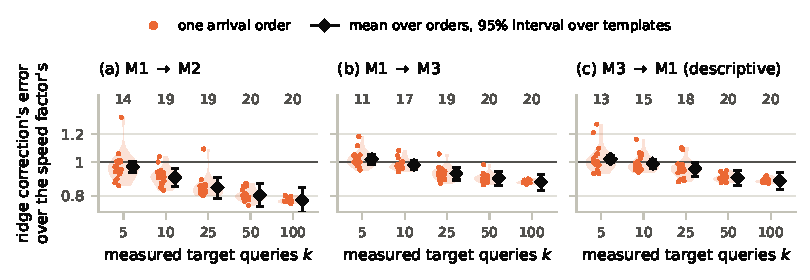
\includegraphics[width=\textwidth]{fig_orders.pdf}
\caption{Q1's comparison, order by order: the ridge correction's error over the speed factor's in each of the \EvalOrders{} arrival orders (dots, violins), and the mean with its 95\% interval over templates (diamonds). Above each violin: orders in which the ridge correction is better.}
\label{fig:orders}
\end{figure}

\textbf{Template offsets.} The ridge correction follows the shift only as far as the features describe it (Section~\ref{sec:shift}). Table~\ref{tab:methods} compares all methods over the 30 pairs of each workload at the budget where each template can have one measured query. With round-robin selection, template offsets reach \PLadTpchTemplateRawRoundRobin{} on TPC-H and \PLadTpcdsTemplateRawRoundRobin{} on TPC-DS and the template correction \PLadTpchLowdimTemplateRoundRobin{} and \PLadTpcdsLowdimTemplateRoundRobin, against \PLadTpchLowdimTemplateControlRoundRobin{} and \PLadTpcdsLowdimTemplateControlRoundRobin{} for the same correction on a model trained on the target itself: once every template has a query, the move costs little. At $k=25$ the template correction reaches \RTcMOneMThree{} (M1 to M3) and \RTcMOneMTwo{} (M1 to M2) against \RRidgeMOneMThree{} and \RRidgeMOneMTwo{} for the ridge correction with random selection (ratios \RTcVsRidgeMOneMThree{} [\RTcVsRidgeMOneMThreeLo, \RTcVsRidgeMOneMThreeHi] and \RTcVsRidgeMOneMTwo{} [\RTcVsRidgeMOneMTwoLo, \RTcVsRidgeMOneMTwoHi]) and closes a share \RTcGapMOneMThree{} of the gap from M1 to M3, where the ridge correction needs $k=\RRidgeNinetyMOneMThree$ to close 0.9. Its interval against the ridge correction lies below 1 in \RTcBelowRidgeTpch{} of \RPairsTpch{} TPC-H ($k=25$) and \RTcBelowRidgeTpcds{} of \RPairsTpcds{} TPC-DS pairs ($k=100$). 1-NN on the same queries does as well, and a forest on the errors beats the ridge correction on TPC-DS (\PLadTpcdsForestResidRandom). A lookup without a model does worse (\PLadTpchLookupRoundRobin{} on TPC-H), and the two refits lose even to the template correction with random selection (\PLTpchKTwoFiveRandomLowdimTemplate).
\begin{table}[t]
\caption{Error at the budget that allows one query per template, geometric mean over the 30 ordered pairs of a workload. Last row: the template correction on a model trained on the target itself (no move), over the six environments.}
\label{tab:methods}
\centering\small
\inputif{results/report/table_methods.tex}
\end{table}

\textbf{TPC-DS and small budgets.} By intervals, on TPC-DS the ridge correction is worse than the speed factor in \RRidgeAboveTpcdsKFive{} of 30 pairs at $k=5$ and \RRidgeAboveTpcdsKOneZero{} at $k=10$, and better in \RRidgeBelowTpcdsKTwoFive, \RRidgeBelowTpcdsKFiveZero{} and \RRidgeBelowTpcdsKOneZeroZero{} at $k=25$, 50 and 100 (Figure~\ref{fig:overview}c); on TPC-H it is better in \RRidgeBelowTpchKTwoFive{} at $k=25$. With at most 4 parameters, affine+parallel is safer before every template has a query: at $k=10$ it beats the speed factor in \PAffTPCHBelow{} TPC-H pairs and loses in \PAffTPCHAbove, and wins in \PAffTPCDSBelow{} and loses in \PAffTPCDSAbove{} on TPC-DS.

\subsection{Which queries to measure}
Covering the templates matters about as much as the correction: on TPC-H at $k=25$, round robin takes the ridge correction from \PLTpchKTwoFiveRandomRidge{} to \PLTpchKTwoFiveRoundRobinRidge{} and the template correction from \PLTpchKTwoFiveRandomLowdimTemplate{} to \PLTpchKTwoFiveRoundRobinLowdimTemplate. Without template labels, k-center selection with 1-NN comes close on TPC-H (\PLTpchKTwoFiveKCenterOneNn) and matches the template correction on TPC-DS at $k=100$ (\PLTpcdsKOneZeroZeroKCenterOneNn{} against \PLTpcdsKOneZeroZeroRoundRobinLowdimTemplate), since queries of one template have near plans. D-optimal selection picks long TPC-DS queries (\PLTpcdsKOneZeroZeroDOptimalCalibrationS\,s of runtime against \PLTpcdsKOneZeroZeroRoundRobinCalibrationS\,s for round robin), and the cheapest query per template saves time but costs accuracy (\PLTpchKTwoFiveRrCheapLowdimTemplate{} on TPC-H), since short queries shift differently. If each of the $k$ queries is timed once, even by its warm-up run, instead of by its three-pass label, the template correction still reaches \SingleTpchFirstLowdimTemplate{} (TPC-H) and \SingleTpcdsFirstLowdimTemplate{} (TPC-DS), and the no-move control rises about as much (\SingleTpchFirstControl{} and \SingleTpcdsFirstControl).

\subsection{C3: continued learning}
Over the whole pool, refitting the ridge correction on all target queries reaches \CThreeMOneMThreeAllPool{} (M1 to M3) and \CThreeMOneMTwoAllPool{} (M1 to M2), against \CThreeMOneMThreeLastPool{} and \CThreeMOneMTwoLastPool{} for the last 50. In a stream that switches from M1 to M2 without warning, scored test-then-train over \EvalStreamOrders{} orders, the error jumps from \CThreeStreamLastBefore{} to \CThreeStreamLastAfter; refitting on the last 50 recovers within \CThreeStreamLastRecover{} queries and ends at \CThreeStreamLastFinal, refitting on all queries at \CThreeStreamAllFinal, and never updating at \CThreeStreamNeverFinal. Over the extended study's \StreamPairs{} streams the template correction on the last 50 ends at \StreamFinalLowdimTemplateLastFiveZero, the ridge correction at \StreamFinalRidgeLastFiveZero{} (last 50) and \StreamFinalRidgeAll{} (all), and no updating at \StreamFinalNever.

\subsection{Q2: unseen templates}
\label{sec:unseen}
\begin{figure}[t]
\centering
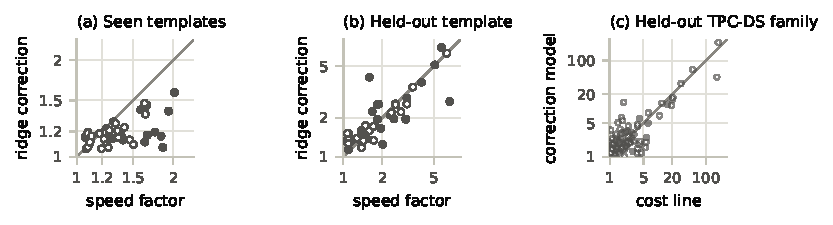
\includegraphics[width=\textwidth]{fig_unseen.pdf}
\caption{Median Q-error per TPC-H template at $k=25$ (a, b; filled: M1$\to$M2, hollow: M1$\to$M3) and per TPC-DS family in C4 (c; filled: families of several templates); below the diagonal the learned correction wins. (a) Seen templates; (b) a template held out of the source model and the $k$ queries; (c) a held-out family.}
\label{fig:unseen}
\end{figure}
On seen templates the ridge correction lowers most errors (Figure~\ref{fig:unseen}a), but on a template held out of the source model and the $k=25$ queries it gains nothing over the speed factor (b): the ratio is \CTwoHardMOneMThreeRvsS{} (\CTwoHardMOneMThreeRvsSLo{} to \CTwoHardMOneMThreeRvsSHi) from M1 to M3 and \CTwoHardMOneMTwoRvsS{} (\CTwoHardMOneMTwoRvsSLo{} to \CTwoHardMOneMTwoRvsSHi) from M1 to M2, and over all pairs of the extended study its interval is never below 1 and is above 1 in \RHardRidgeAboveTpch{} TPC-H and \RHardRidgeAboveTpcds{} TPC-DS pairs. Retraining helps little: the speed factor is within \PHHFourMaxAll{} times the error of the oracle retrained without the template in every pair, so what remains is the model's error on a new template.

Q2's primary test fails (Figure~\ref{fig:unseen}c): with one TPC-DS family held out at a time, the correction model's error is \CFourGeo{} times the cost line's (95\% interval \CFourGeoLo{} to \CFourGeoHi), better on \CFourWins{} of \CFourN{} families, and both do poorly (median Q-errors \CFourHybMed{} and \CFourCostMed, 90th percentiles \CFourHybPninety{} and \CFourCostPninety). Holding out single templates flatters the correction model, \CFourTplGeo{} (\CFourTplGeoLo{} to \CFourTplGeoHi), because a near copy of the held-out template stays in training; even so the interval contains 1.

\subsection{Confirmatory tests and other source models}
\label{sec:confirm}
The five hypotheses fixed before the \PHPairs{} new pairs existed hold under their registered rules: (H1) the template share exceeds 0.5 in every pair (smallest \PHHOneMin); (H2) at $k=100$ the template correction with round robin beats the speed factor in \PHHTwoVsSpeedOk{} of \PHHTwoN{} pairs and the ridge correction with random selection in \PHHTwoVsRidgeOk; (H3) at $k=10$ affine+parallel beats the speed factor in \PHHThreeOk{} of \PHHThreeN{} pairs between one processor and several, meeting the registered three quarters (\PHHThreeOkCI{} by intervals); (H4) on new templates the speed factor is within 1.15 times the oracle's error (largest \PHHFourMax); (H5) at $k=100$ k-center with 1-NN beats random selection with the ridge correction in \PHHFiveOk{} of \PHHFiveN{} pairs (\PHHFiveOkCI{} by intervals). With a random forest, boosted trees, ridge regression or the cost line as $f_s$, the template correction beats the speed factor in all \SrcWinsTotal{} combinations of source model, workload and pair.

\section{Discussion and Limitations}
For a database that moves to a new machine, the results suggest a recipe: measure one query of each template that matters, chosen round robin, and add to the old model a per-template offset on top of a line that treats parallel plans separately. In the terms of Section~\ref{sec:setup}, the shift $\delta$ is mostly a per-template effect: one measured query estimates a template's offset, and the source model supplies the variation inside the template. This came within about 2\% of the same correction on a model trained on the new machine, for about \PLTpchKTwoFiveRoundRobinCalibrationS\,s of TPC-H runtime. The ridge correction proposed for this course beats a speed factor on TPC-H after 10 to 25 queries but on TPC-DS only from about 50, because the features describe only part of the shift.

The study uses one database system at scale factor 1 (data in memory), queries under 30\,s run warm and one at a time, and two physical x86 machines, both virtualized; the 30 pairs of a workload reuse six environments' labels, so they are not independent replications. Plans were held fixed, while a real move may change them, and pinning keeps two workers per Gather node. Errors are per-template medians, and only C4 reports tails. I designed the template methods after seeing the TPC-H pairs among M1 to M3, which is why they were confirmed on pairs measured later.

\section{Conclusion}
A runtime model moved to a new machine needs no new training set: on TPC-H a ridge correction from 25 measured queries beats a speed factor (Q1), and one query per template with a per-template offset comes close to a model trained there. On a template without measured queries no correction reliably beats the speed factor, and the cost-anchored model is no better than the cost line (Q2). Next steps are other database systems, larger data and plans that change with the machine.

\clearpage
\section*{Acknowledgement}
% The author writes this section.

\renewcommand*{\bibfont}{\small}
\setlength{\bibitemsep}{0.3\baselineskip}
\printbibliography[title=References]
\end{document}
